\documentclass[12pt]{article}
\usepackage[russian]{babel}
\usepackage{amsmath}
\usepackage{amsfonts}
\usepackage{amssymb}
\usepackage{mathtools}
\usepackage{graphicx}
\usepackage{xcolor}
\selectcolormodel{gray}
\usepackage{subfig}
\textwidth 16.5cm \textheight 23cm \topmargin -1.5cm
\usepackage{algorithm}% http://ctan.org/pkg/algorithms
\captionsetup[algorithm]{labelformat=empty}
\usepackage[noend]{algpseudocode}
\usepackage{hyperref}

\newtheorem{theorem}{Теорема}
\newtheorem{lemma}{Лемма}
\newtheorem{corollary}{Следствие}
\newtheorem{definition}{Определение}
\newtheorem{remark}{Замечание}
\newtheorem{problem}{Задача}
\renewcommand{\div}{\mathop{\mathrm{div}}\nolimts}
\renewcommand\thesubfigure{\asbuk{subfigure}}
\usepackage{caption}
\usepackage{textcomp}
\captionsetup[figure]{labelsep=period}


\begin{document}
    \def\figurename{Фиг.}
    %\Large
    УДК 517.95
    \begin{center}
        \textbf{ ГРАНИЧНАЯ ОБРАТНАЯ ЗАДАЧА СЛОЖНОГО ТЕПЛООБМЕНА }
        \footnote[{1}]{$^)$Работа выполнена при финансовой поддержке РФФИ (код проекта 20-01-00113) и ИПМ ДВО РАН
            (НИОКТР \textnumero~АААА-А20-120120390006-0)}$^)$
    \end{center}
    \begin{center}
        \textbf{ \copyright\  2022 г.\ \  П.Р. Месенев, А.Ю. Чеботарев$^{*}$}
        \\
        \textit{ 690041 Владивосток,ул.Радио,7,ИПМ ДВО РАН;\\ 690922 Владивосток, о. Русский, п. Аякс, 10, ДВФУ,
            Региональный научно-образовательный центр -- Дальневосточный центр математических исследований\\
            e-mail:  $^{*}$cheb@iam.dvo.ru}\\
        {\small  Поступила в редакцию \\ Переработанный вариант\\
        Принята к публикации }
    \end{center}

    \sloppy
    \begin{quote}
        \small
        Рассмотрена граничная обратная задача для стационарных уравнений сложного теплообмена с незаданным краевым условием для интенсивности излучения на части границы и условием переопределения на другой части границы.
        Предложен оптимизационный метод решения обратной задачи и представлен анализ соответствующей задачи
        граничного оптимального управления.
        Показано, что последовательность решений экстремальных задач
        сходится к решению обратной задачи.
        Эффективность алгоритма проиллюстрирована численными примерами.
        Библ.
        32.
    \end{quote}
    \textbf{ Ключевые слова:} уравнения радиационно-кондуктивного теплообмена, диффузионное
    приближение, обратная задача, задача оптимального управления.

    \begin{center}
        \textbf{1. ПОСТАНОВКА ОБРАТНОЙ ЗАДАЧИ}
    \end{center}

    Рассмотрим следующую систему полулинейных эллиптических уравнений, которая
    моделирует радиационный и диффузионный (сложный) теплообмен в
    ограниченной липшицевой области $\Omega\subset \mathbb{R}^3$ с границей
    $\Gamma=\partial\Omega$ ~\cite{Pinnau07}-\cite{Kovt14-1}.
    \begin{equation}
        \label{eq1}
        - a\Delta\theta + b\kappa_a(|\theta|\theta^3- \varphi)=0,   \quad
        -\alpha \Delta \varphi + \kappa_a(\varphi-|\theta|\theta^3)=0,\; x\in\Omega.
    \end{equation}
    Через $\theta$ и $\varphi$ здесь обозначены температура и усредненная по всем
    направлениям интенсивность теплового излучения. Положительные параметры
    $a$, $b$, $\kappa_a$ и $\alpha$, описывающие
    свойства среды, являются заданными~\cite{Kovt14-1}.


    Пусть граница области состоит из двух участков, $\Gamma \coloneqq \partial \Omega =\overline{\Gamma}_1 \cup \overline{\Gamma}_2$,
    так что $\Gamma_1 \cap \Gamma_2 =  \emptyset$.
    На всей границе $\Gamma$ задается тепловой поток $q_b$,
    \begin{equation}
        \label{bc1}
        a\partial_n\theta = q_b, \quad x\in \Gamma.
    \end{equation}
    Для задания краевого условия для интенсивности излучения
    требуется знать функцию $\gamma$, описывающую отражающие свойства границы \cite{JVM-14}.
    В случае, если эта функция неизвестна на части границы $\Gamma_2$,
    краевое условие для интенсивности излучения на $\Gamma_2$ не ставится, а в качестве условия переопределения на $\Gamma_1$, в дополнение к условию на
    $\varphi$, задается температурное поле $\theta_b$,
    \begin{equation}
        \label{bc2}
        \alpha\partial_n\varphi + \gamma (\varphi - \theta_b ^4 ) = 0,\;\;
        \theta=\theta_b\quad x\in \Gamma_1.
    \end{equation}
    Здесь через $\partial_n$ обозначаем производную в направлении
    внешней нормали $\mathbf n$.

    В данной работе предлагается оптимизационный метод решения задачи~\eqref{eq1}-\eqref{bc2}, который заключается в рассмотрении задачи граничного оптимального управления для эквивалентной системы эллиптических уравнений.
    Для постановки задачи управления введем новую неизвестную функцию
    $\psi= a\theta + \alpha b \varphi$. Складывая первое уравнение в \eqref{eq1} со вторым, умноженным на $b$, заключаем, что $\psi$ -- гармоническая функция.
    Исключая $\varphi$ из первого уравнения в \eqref{eq1} и используя краевые условия
    \eqref{bc1},\eqref{bc2},  получаем краевую задачу
    \begin{equation}
        \label{eq2}
        - a \Delta \theta + g (\theta) = \frac{\kappa_a}{\alpha}\psi, \quad
        \Delta \psi = 0, \; x \in \Omega,
    \end{equation}
    \begin{equation}
        \label{bc3}
        a \partial_n \theta = q_b, \; \text{ на }\Gamma, \;\;
        \alpha \partial_n \psi + \gamma \psi  =  r,\;\;
        \theta = \theta_b  \text{ на }\Gamma_1.
    \end{equation}
    Здесь $g(\theta) = b \kappa_a|\theta|\theta^3 + \frac{a\kappa_a}{\alpha}\theta$, $r=\alpha b \gamma \theta_b^4+ \alpha q_b + a \gamma \theta_b$.

    Сформулируем задачу оптимального управления, которая аппроксимирует задачу~\eqref{eq2},\eqref{bc3}.
    Задача состоит в отыскании тройки $\{\theta_\lambda,\psi_\lambda,u_\lambda\}$ такой, что
    \begin{equation}
        \label{cost}
        \begin{split}
            J_\lambda(\theta, u) = \frac{1}{2}\int\limits_{\Gamma_1} (\theta - \theta_b)^2d\Gamma + \frac{\lambda}{2}\int\limits_{\Gamma_2} u^2d\Gamma \rightarrow\inf, \\
            - a \Delta \theta + g (\theta) = \frac{\kappa}{\alpha}\psi, \quad
            \Delta \psi = 0, \; x \in \Omega,\\
            a \partial_n \theta + s \theta = q_b + s\theta_b, \; \alpha \partial_n \psi + \gamma \psi = r, \text{ на } \Gamma_1,\;\; a \partial_n \theta  = q_b,\;
            \alpha \partial_n \psi = u \text{ на } \Gamma_2.
        \end{split}
    \end{equation}
    Здесь $\lambda, s > 0$ -- регуляризирующие параметры.


    Нелинейные модели сложного теплообмена в рамках $P_1$ приближения для уравнения переноса теплового
    излучения достаточно полно изучены.
    В работах~\cite{Pinnau07}-\cite{JVM-19-INV} представлены постановки и анализ различных краевых,
    обратных и экстремальных задач для таких моделей.
    Интересные результаты анализа краевых задач сложного теплообмена,
    без использования $P_1$ приближения, получены в~\cite{Amosov16}-\cite{Amosov20-1}.


    \begin{center}
        \textbf{2. РАЗРЕШИМОСТЬ ЗАДАЧИ ОПТИМАЛЬНОГО УПРАВЛЕНИЯ}
    \end{center}

    Рассмотрим пространства $H = L^2(\Omega), \; V = H^1(\Omega)=W^1_2(\Omega)$, $V'$ -- пространство, сопряженное с $V$.
    Пространство $H$ отождествляем с пространством $H'$ так, что $V \subset H = H' \subset V'$. Через $U$ обозначаем пространство управлений $L^2(\Gamma_2)$.
    Стандартную норму в $H$ обозначаем $\|\cdot\|$,
    $(f,v)$ -- значение функционала $f\in V'$ на элементе $v\in V$,
    совпадающее со скалярным произведением в $H$, если $f\in H$.


    Будем предполагать, что исходные данные удовлетворяют условиям:

    (i) $\;\; a,b,\alpha,\kappa_a, \lambda, s ={\rm Const}> 0 ,$

    (ii) $\;\,0<\gamma_0\leq \gamma\in L^\infty(\Gamma_1),\,\theta_b, r \in L^2(\Gamma_1),\;\; q_b\in L^2(\Gamma).$


    Определим операторы $A_{1,2}\colon V \to V'$, $B_1\colon L^2(\Gamma_1)\to V'$,
    $B_2\colon U\to V'$ используя
    равенства, справедливые для любых $y,z \in V$, $f,v\in L^2(\Gamma_1)$,
    $h,w\in U$:
    \[
        (A_1y,z) =a (\nabla y, \nabla z) +
        s\int\limits_{\Gamma_1}yz d\Gamma, \;\;
        (A_2y,z) =\alpha (\nabla y, \nabla z) +
        \int\limits_{\Gamma_1}\gamma yz d\Gamma,
    \]
    $$
    (B_1f, v)
    = \int\limits_{\Gamma_1}fv d\Gamma,\;\; (B_2h, w)
    = \int\limits_{\Gamma_2}hw d\Gamma.
    $$
    Заметим, что
    билинейная форма $(A_1y,z)$ определяет скалярное произведение
    в пространстве $V$ и норма $\|z\|_V=\sqrt{(A_1z,z)}$ эквивалентна
    стандартной норме $V$. Кроме того, определены непрерывные обратные
    операторы
    $A_{1,2}^{-1}:\,V'\mapsto V.$ Для
    $y\in V$, $f\in L^2(\Gamma_1)$, $h\in V'$ справедливы неравенства
    \begin{equation}
        \label{E}
        \|y\|\leq K_0\|y\|_V,\; \; \|B_1f\|_{V'}\leq K_1\|w\|_{L^2(\Gamma_1)},
        \;\;
        \|B_2 h\|_{V'}\leq K_2\|h\|_{U}.
    \end{equation}
    Здесь постоянные $K_j>0$ зависят только от области $\Omega.$

    Используя введенные операторы, слабую формулировку краевой задачи, на решениях которой минимизируется функционал \eqref{cost}, нетрудно записать в виде
    \begin{equation}
        \label{CS}
        A_1\theta+g(\theta)=\frac{\kappa_a}{\alpha}\psi+f_1,\;\;\; A_2\psi=f_2+B_2u,
    \end{equation}
    где $f_1=B_1(q_b+s\theta_b)+B_2q_b$, $f_2=B_1r.$

    Для формализации задачи оптимального управления
    определим оператор
    ограничений $F(\theta, \psi, u) : V \times V \times U \rightarrow V' \times V'$,
    \[
        F(\theta, \psi, u) = \{A_1\theta+g(\theta)-\frac{\kappa_a}{\alpha}\psi-f_1 ,\;
        A_2\psi-f_2-B_2u, \}.
    \]


    \textbf{Задача $(P_\lambda)$.} Найти тройку $\{\theta_\lambda, \psi_\lambda, u_\lambda \} \in V \times V \times U$
    такую, что
    \begin{equation}
        \label{CP}
        J_\lambda(\theta, u) = \frac{1}{2}\|\theta -\theta_b\|^2_{L^2(\Gamma_1)}
        + \frac{\lambda}{2}\|u\|^2_U \rightarrow \text{inf},\;\; F(\theta, \psi, u)=0.
    \end{equation}

    \textbf{Лемма 1.}
    \textit{
        Пусть выполняются условия} (i),(ii), $u\in U$. \textit{ Тогда
    существует единственное решение системы~\eqref{CS} и при этом}
    \begin{equation}
        \label{E1}
        \begin{aligned}
            \|\theta\|_V \leq
            \frac{K_0^2\kappa_a}{\alpha}\|\psi\|_V+\|f_1\|_{V'}, \\
            \|\psi\|_V\leq \|A_2^{-1}\|\left(\|f_2\|_{V'}+K_2\|u\|_U\right).
        \end{aligned}
    \end{equation}

    \textbf{ Доказательство.}
    Из второго уравнения в \eqref{CS} следует, что $\psi=A_2^{-1}(f_2+B_2u)$  и поэтому
    $$
    \|\psi\|_V\leq \|A_2^{-1}\|\left(\|f_2\|_{V'}+K_2\|u\|_U\right).
    $$
    Однозначная разрешимость первого уравнения~\eqref{CS} с монотонной нелинейностью хорошо известна (см.
    например~\cite{Kufner}). Умножим скалярно это уравнение на
    на $\theta $, отбросим неотрицательное
    слагаемое $(g(\theta),\theta)$ и оценим правую часть, используя неравенство Коши-Буняковского.
    Тогда, с учетом неравенств \eqref{E}, получаем
    \[
        \|\theta\|^2_V \leq \frac{\kappa_a}{\alpha}\|\psi\|\|\theta\|+\|f_1\|_{V'}\|\theta\|_V\leq
        \frac{K_0^2\kappa_a}{\alpha}\|\psi\|_V\|\theta\|_V+\|f_1\|_{V'}\|\theta\|_V
    \]
    В результате получаем оценки~\eqref{E1}.

    \textbf{Теорема 1.}
    \textit{
        При выполнении условий} (i),(ii)
    \textit{ существует решение задачи $(P_\lambda).$
    }

    \textbf{ Доказательство.}
    Обозначим через
    $j_\lambda $ точную нижнюю грань целевого функционала $J_\lambda$
    на множестве $u \in U$, $F(\theta, \psi, u)=0$ и рассмотрим
    последовательности такие, что
    $u_m \in U, \; \theta_m \in V, \;\psi_m\in V$, $J_\lambda(\theta_m, u_m)
    \rightarrow j_\lambda,$
    \begin{equation}
        \label{MS}
        A_1\theta_m+g(\theta_m)=\frac{\kappa_a}{\alpha}\psi_m+f_1,\;\;\; A_2\psi_m=f_2+B_2u_m.
    \end{equation}
    Из ограниченности последовательности $u_m$ в пространстве $U$ следуют, на основании
    леммы 1, оценки
    \[
        \|\theta_m\|_V \leq C,\;\;
        \|\psi_m\|_V \leq C,\;\;\|\theta_m\|_{L^6(\Omega)} \leq C.
    \]
    Здесь через $C>0$ обозначена наибольшая из постоянных, ограничивающих соответствующие нормы и не зависящих от $m$.
    Переходя при необходимости к подпоследовательностям, заключаем, что
    существует тройка $\{ \hat{u}, \hat{\theta}, \hat{\psi} \} \in U \times V \times V,$
    \begin{equation}
        \label{L}
        u_m \rightarrow \hat{u} \text{  слабо в } U, \;\;
        \theta_m, \psi_m \rightarrow \hat{\theta}, \hat{\psi} \text{
            слабо в } V, \text{
            сильно в } L^4(\Omega).
    \end{equation}
    Заметим также, что $\forall v \in V$ имеем
    \begin{equation}
        \label{L1}
        |( [\theta_m]^4 - [\hat{\theta}]^4, v)|
        \leq 2 \| \theta_m - \hat{\theta}\|_{L^4(\Omega)} \|v\|_{L^4(\Omega)}
        \left( \| \theta_m \|^3_{L_6(\Omega)} + \| \hat{\theta} \|^3_{L_6(\Omega)}\right).
    \end{equation}
    Результаты о сходимости~\eqref{L} и неравенство \eqref{L1} позволяют перейти
    к пределу в~\eqref{MS}. В результате получим
    \begin{equation}
        \label{w1}
        A_1 \hat{\theta} + g(\hat{\theta}) = \frac{\kappa_a}{\alpha}\hat{\psi}+f_1,\;\;\; A_2\hat{\psi}=f_2+B_2\hat{u}.
    \end{equation}
    Поскольку целевой функционал слабо полунепрерывен снизу, то   $j_\lambda \leq J_\lambda(\hat{\theta}, \hat{u}) \leq \varliminf J_\lambda(\theta_m, u_m) =
    j_\lambda$ и поэтому
    тройка $\{\hat{\theta}, \hat{\psi}, \hat{u} \}$ есть
    решение задачи $(P_\lambda).$

    \begin{center}
        \textbf{4. УСЛОВИЯ ОПТИМАЛЬНОСТИ ПЕРВОГО ПОРЯДКА}
    \end{center}

    Воспользуемся принципом
    Лагранжа для гладко-выпуклых экстремальных задач~\cite{10},\cite{11}. Невырожденность условий оптимальности гарантируется условием, что
    образ производной
    оператора ограничений $F(y, u)$, где $y=\{\theta,\psi\}\in V\times V$,
    совпадает с пространством $V'\times V'.$  Последнее означает, что
    линейная система
    $$
    A_1\xi+g'(\theta)\xi-\frac{\kappa_a}{\alpha}\eta=q_1,\quad
    A_2\eta=q_2
    $$
    разрешима для всех $\theta\in V$, $q_1,q_2\in V'.$ Здесь
    $g'(\theta)=4b\kappa_a|\theta|^3+\frac{\kappa_a}{\alpha}.$
    Из второго уравнения получаем $\eta=A_2^{-1}q_2.$ Разрешимость первого уравнения при известном $\eta\in V$ очевидным образом следует из леммы Лакса--Мильграма. Отметим, что справедливость остальных условий принципа Лагранжа также очевидна.

    Функция Лагранжа задачи $(P_\lambda)$
    имеет вид
    \[
        L(\theta, \psi, u, p_1, p_2) = J_\lambda(\theta, u)
        + (A_1\theta+g(\theta)-\frac{\kappa_a}{\alpha}\psi-f_1 ,p_1)+
        (A_2\psi-f_2-B_2u,p_2),
    \]
    где $p=\{p_1,p_2\}\in V\times V$ -- сопряженное состояние.

    Пусть $\{\hat{\theta}, \hat{\varphi}, \hat{u} \}$ -- решение задачи
    $(P_\lambda)$. Вычислив производные Гато функции Лагранжа по $\theta,\,\psi$ и $u$, получаем
    в силу принципа Лагранжа~\cite[Теорема 1.5]{10} следующие равенства
    $\forall v\in V,\, w\in U$
    \begin{equation}
        \label{OC1}
        (B_1(\hat{\theta} -\theta_b), v) + (A_1v+g'(\hat{\theta})v,p_1)=0,\;
        -\frac{\kappa_a}{\alpha}(v ,p_1)+
        (A_2v,p_2),    = 0,
    \end{equation}
    \begin{equation}
        \label{OC2}
        \lambda(B_2\hat{u},w) - (B_2w, p_2) = 0.
    \end{equation}
    Из условий~\eqref{OC1},\eqref{OC2} вытекают уравнения для сопряженного состояния, которые вместе с уравнениями \eqref{w1}
    для оптимальной тройки дают систему оптимальности задачи $(P_\lambda)$.

    \textbf{Теорема 2.}
    \textit{ Пусть выполняются условия} (i),(ii).
    \textit{ Если $\{\hat{\theta}, \hat{\psi}, \hat{u}\}$ -- решение
    задачи $(P_\lambda)$, то существует единственная пара $\{p_1, p_2 \} \in V\times V$
        такая, что}
    \begin{equation}
        \label{AS}
        A_1p_1+g'(\hat{\theta}) p_1=-B_1(\hat{\theta} -\theta_b),\;\;
        A_2p_2=\frac{\kappa_a}{\alpha}p_1,\;\;
        \lambda\hat{u}=p_2|_{\Gamma_2}.
    \end{equation}

    \textbf{Замечание.} Если рассмотреть приведенный целевой функционал $\tilde J_\lambda(u)=J_\lambda(\theta(u), u)$, где $\theta(u)$ компонента решения
    задачи~\eqref{CS}, соответствующая управлению $u\in U$,
    то градиент функционала $\tilde J_\lambda(u)$ равен
    $ \tilde J'_\lambda (u) = \lambda u - p_2. $
    Здесь $p_2$ -- компонента решения сопряженной системы \eqref{AS},
    где $\hat{\theta}\coloneqq\theta(u)$.


    \begin{center}
        \textbf{5. АППРОКСИМАЦИЯ РЕШЕНИЯ ОБРАТНОЙ ЗАДАЧИ}
    \end{center}

    Покажем, что если существует пара $\{\theta,\varphi\}\in V\times V$
    --
    решение обратной задачи \eqref{eq1}-\eqref{bc2} и при этом
    $q=a\partial_n\varphi|_{\Gamma_2}\in L^2(\Gamma_2)$, то
    решения задачи $(P_\lambda)$ при $\lambda\to+0$
    аппроксимируют решение задачи~\eqref{eq1}-\eqref{bc2}.

    Предварительно заметим, что указанная пара для всех $v\in V$ удовлетворяет равенствам
    \begin{equation}
        \label{IP1}
        a(\nabla\theta, \nabla v) + b\kappa_a(|\theta|\theta^3- \varphi ,v)=\int\limits_\Gamma q_bvd\Gamma ,
    \end{equation}
    \begin{equation}
        \label{IP2}
        \alpha (\nabla \varphi,\nabla v)+\int\limits_{\Gamma_1}\gamma\varphi vd\Gamma + \kappa_a(\varphi-|\theta|\theta^3,v)=
        \int\limits_{\Gamma_1}\gamma\theta_b^4 vd\Gamma +\int\limits_{\Gamma_2}q vd\Gamma
    \end{equation}
    и при этом $\theta|_{\Gamma_1}=\theta_b.$

    \textbf{Теорема 3.}
    \textit{
        Пусть выполняются условия} (i),(ii) \textit{ и существует решение задачи~\eqref{eq1}-\eqref{bc2}, удовлетворяющее равенствам \eqref{IP1}, \eqref{IP2}},
    \textit{  Если $\{\theta_\lambda,\psi_\lambda,u_\lambda\}$ -- решение
    задачи $(P_\lambda)$ для $\lambda>0$, то существует последовательность
        $\lambda\to +0$
        такая, что}
    \[
        \theta_\lambda\rightarrow\theta_*, \;\;
        \frac{1}{\alpha b}(\psi_\lambda-a\theta_\lambda)\rightarrow\varphi_*
        \text{ \textit{ слабо в} }V,\text{ \textit{ сильно в} }H,
    \]
    \textit{ где $\theta_*,\varphi_*$ -- решение задачи~\eqref{eq1}-\eqref{bc2}.}

    \textbf{ Доказательство.}
    Умножим равенство \eqref{IP1} на $\alpha$, \eqref{IP2} на $\alpha b$
    и сложим равенства. Тогда, полагая $\psi=a\theta+\alpha b\varphi$,
    $u=\alpha bq+\alpha q_b|_{\Gamma_2}$, получаем
    $$
    \alpha(\nabla\psi,\nabla v)+\int\limits_{\Gamma_1}\gamma\psi vd\Gamma =
    \int\limits_{\Gamma_1}r vd\Gamma +\int\limits_{\Gamma_2}u vd\Gamma.
    $$
    Здесь $r=\alpha b \gamma \theta_b^4+ \alpha q_b + a \gamma \theta_b.$
    Поэтому $A_2\psi=f_2+B_2u.$

    Из \eqref{IP1}, с учетом условия $\theta|_{\Gamma_1}=\theta_b$ выводим равенство $A_1\theta +g(\theta)=\frac{\kappa_a}{\alpha}\psi+f_1.$
    Таким образом, тройка $\{\theta, \psi, u\} \in V \times V \times U$ является допустимой для задачи $(P_\lambda)$ и следовательно
    \[
        J_\lambda(\theta_\lambda, u_\lambda) = \frac{1}{2}\|\theta_\lambda -\theta_b\|^2_{L^2(\Gamma_1)}
        + \frac{\lambda}{2}\|u_\lambda\|^2_U\leq J_\lambda(\theta, u)=\frac{\lambda}{2}\|u\|^2_U.
    \]
    Тогда
    \[
        \|u_\lambda\|^2_U\leq \|u\|^2_U,\;\; \|\theta_\lambda -\theta_b\|^2_{L^2(\Gamma_1)}\to 0,\; \lambda\to +0.
    \]
    Из ограниченности последовательности $u_\lambda$ в пространстве $U$ следуют, на основании
    леммы 1, оценки
    \[
        \|\theta_\lambda\|_V \leq C,\;\;
        \|\psi_\lambda\|_V \leq C,
    \]
    где постоянная $C>0$ не зависит от $\lambda.$
    Поэтому можно выбрать последовательность $\lambda\to+0$ такую, что
    \begin{equation}
        \label{LL}
        \begin{split}
            u_\lambda \rightarrow u_* \text{ \textit{  слабо в} } U, \;\;
            \theta_\lambda, \psi_\lambda \rightarrow \theta_*,\psi_* \text{
                \textit{ слабо в} } V, \text{
                \textit{ сильно в} } H,L^4(\Omega),\\
            \theta_\lambda|_{\Gamma_1}\rightarrow
            \theta_*|_{\Gamma_1} \text{ \textit{ сильно в } }L^2(\Gamma_1).
        \end{split}
    \end{equation}
    Результаты~\eqref{LL} позволяют перейти к пределу при $\lambda\to+0$
    в уравнениях для $\theta_\lambda,\psi_\lambda,u_\lambda$ и тогда
    \begin{equation}
        \label{CC}
        A_1 \theta_* + g(\theta_*) = \frac{\kappa_a}{\alpha}\psi_*+f_1,\quad
        A_2\psi_*  =f_2+ B_2u_*,\quad \theta_*|_{\Gamma_1}=\theta_b.
    \end{equation}
    Полагая $\varphi_*= \frac{1}{\alpha b}(\psi_*-a\theta_*$, заключаем, что
    пара $\theta_*,\varphi_*$ -- решение задачи~\eqref{eq1}-\eqref{bc2}.


    \begin{center}
        \textbf{6. ЧИСЛЕННЫЕ ПРИМЕРЫ}
    \end{center}

    Представим итерационный алгоритм решения задачи оптимального управления.
    Пусть $\tilde J_\lambda(u)=J_\lambda(\theta(u), u)$, где $\theta(u)$ компонента решения
    задачи~\eqref{eq1},\eqref{bc2}, соответствующая управлению $u\in U$.

    В соответствии с~\eqref{AS} градиент функционала $\tilde J_\lambda(u)$ равен
    \[ \tilde J'_\lambda (u) = \lambda u - p_2. \]
    Здесь $p_2$ -- соответствующая компонента сопряженного состояния из системы ~\eqref{AS},
    где $\hat{\theta}\coloneqq\theta(u)$.

    \begin{algorithm}[H]
        \caption{Алгоритм градиентного спуска}
        \label{alg:algorithm}
        \begin{algorithmic}[1]
            \State Выбираем значение градиентного шага $\varepsilon$,
            \State Выбираем количество итераций $N$,
            \State Выбираем начальное приближение для управления $u_0 \in U$,
            \For{$k \gets 0,1,2,\dots,N$}
                \State Для данного $u_k$ рассчитываем состояние $y_k = \{\theta_k, \varphi_k\}$ --
                решение задачи~\eqref{eq1},\eqref{bc1}.
                \State Рассчитываем значение целевого функционала $J_\lambda(\theta_k, u_k)$.
                \State Рассчитываем сопряженное состояние $p_k=\{p_{1k},p_{2k}\}$ из уравнений ~\eqref{OC1},
                где $ \hat{\theta} \coloneqq \theta_k, \hat{u}=u_k$.
                \State Пересчитываем управление $u_{k+1} = u_k - \varepsilon (\lambda u_k - p_2)$
            \EndFor
        \end{algorithmic}
    \end{algorithm}
    Значение параметра $\varepsilon$ выбирается эмпирически таким образом, чтобы значение
    $\varepsilon (\lambda u_k - p_2)$ являлось существенной поправкой для $u_{k+1}$.
    Количество итераций $N$ выбирается достаточным для выполнения условия
    $J_\lambda(\theta_k, u_k) - J_\lambda(\theta_{k+1}, u_{k+1}) < \delta$, где $\delta>0$
    определяет точность расчетов.

    Примеры, рассмотренные ниже, иллюстрируют работоспособность предложенного алгоритма при
    малых, что важно, значениях параметра регуляризации $\lambda \leq 10^{-12}$.
    В первом примере выполнены тестовые расчеты для куба.
    Во втором примере рассмотрен куб с внутренней полостью.
    Для численного решения прямой задачи с заданным управлением использовался
    метод Ньютона для линеаризации задачи и ее решения методом конечных элементов.
    Решение сопряженной системы, которая является линейной при заданной температуре, не вызывает трудностей.
    Для численного моделирования использовался солвер FEniCS~\cite{fenics},\cite{dolfin}.

    Исходный код экспериментов можно найти по ссылке~\cite{mesenev-github}.

    \textbf{Пример 1.}
    Рассмотрим куб $\Omega = {(x, y, z), 0 \leq x,y,z \leq l}$ с границей $\Gamma \equiv \Gamma_1 \cup \Gamma_2$, где
    \[
        \Gamma_1 = \{(x, y, z), 0 \leq x,y, \leq l, z \in 0, l\}, \;
        \Gamma_2 = \partial \Omega \setminus \hat{\Gamma_1}.
    \]
    Будем считать, что
    $l=1~\text{см}$,
    $a = 0.6[\text{см}^2/\text{c}]$,
    $b=0.025[\text{см}/\text{с}]$,
    $\kappa_a=1[\text{см}^{-1}]$,
    $\alpha = 0.(3)[\text{см}]$.
    Указанные параметры соответствуют стеклу~\cite{Grenkin5}.
    Параметр регуляризации $\lambda=10^{-12}$.

    Пусть граничные данные $q_b$ и $\theta_b$ в~\eqref{bc1},\eqref{bc2} имеют вид:
    \begin{gather*}
        q_b = 0.5, \quad
        \theta_b = 0.1 + z/2.
    \end{gather*}
    А также начальное управление $u_0 = 0$.
    Используя предложенный алгоритм~\ref{alg:algorithm} решим задачу оптимального управления.

    \begin{figure}[H]
        \centering
        \subfloat[$|\partial_n \theta_\lambda - q_n|/\ q_n$]
        {
            \label{fig:img_test_1}
            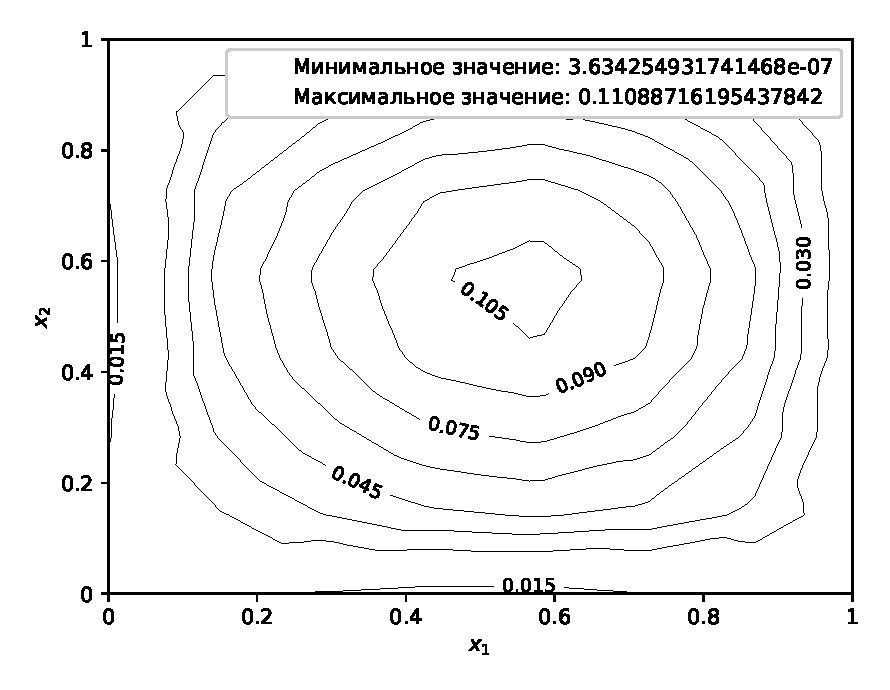
\includegraphics[width=.49\linewidth]{img/exp1_iso}
        }
        \subfloat[Изменение функционала качества по итерациям]
        {
            \label{fig:quality_1}
            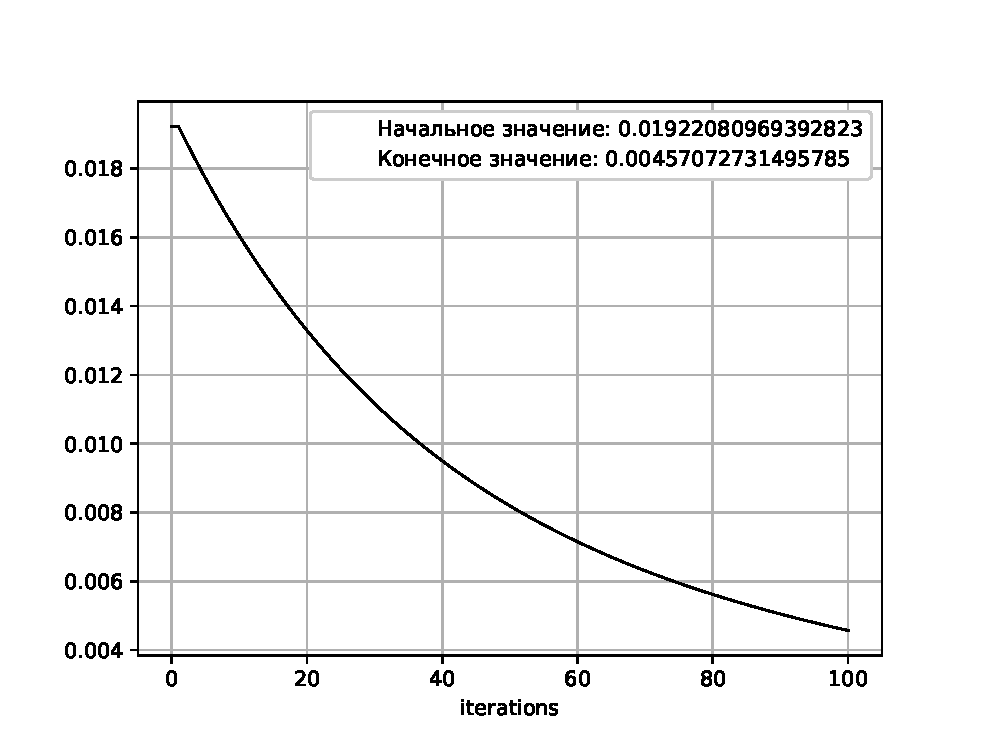
\includegraphics[width=.49\linewidth]{img/exp1_quality}
        }
        \caption{Результаты первого эксперимента}
        \label{fig:1}
    \end{figure}

    \begin{figure}[H]
        \centering
        \subfloat[$\theta|_{x=0.5}$]
        {
            \label{fig:img_slice_1}
            \includegraphics{img/exp1_slice}
        }
        \label{fig:2}
    \end{figure}

    На фиг.~\ref{fig:img_test_1}, \ref{fig:quality_1} представлены модуль относительного
    отклонения $\partial_n\theta_\lambda$ от $q_b$ на грани куба в плоскости $z=l$,
    где $\partial_n\theta_\lambda=\partial\theta_\lambda/\partial z$ и динамика целевого функционала, определяющего норму
    разности $\|\theta_\lambda -\theta_b\|^2_\Gamma$.
    На остальных гранях куба значения относительного отклонения имеют тот же порядок малости.
    На фиг.~\ref{fig:img_slice_1} представлено значение температурного поля в плоскости $x=0.5$.

    \textbf{Пример 2.}
    Рассмотрим единичный куб $C = \{(x, y, z), 0 \leq x,y,z \leq l\}$ с
    шарообразной полостью с центром $b_0 =\{0.5, 0.5, 0.5\}$
    $B = \{r, \| r - b_0 \| \leq 0.15 \}$.
    Рассматриваемая область $\Omega = C \setminus B$.
    $\Gamma \equiv \partial \Omega = \partial C \cup \partial B$ при чём
    \[
        \Gamma_1 = \partial B,
        \Gamma_2 = \partial C.
    \]
    Параметры среды возьмём из примера 1.
    Граничные данные $q_b$ и $\theta_b$ положим равными
    \begin{gather*}
        q_b = 1, \quad
        \theta_b = 0.25.
    \end{gather*}
    \begin{figure}[H]
        \centering
        \subfloat[$|\partial_n \theta_\lambda - q_n|/\ q_n$]
        {
            \label{fig:img_slice_2}
            \includegraphics[width=.5\linewidth]{img/exp3_slice}
        }
        \subfloat[Изменение функционала качества по итерациям]
        {
            \label{fig:img_quality_2}
            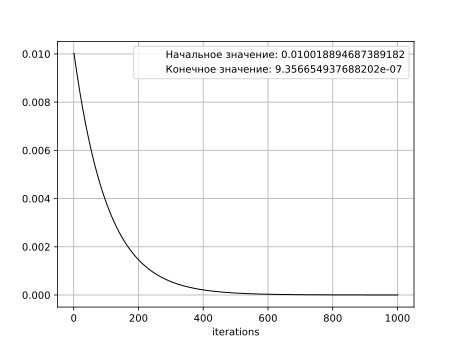
\includegraphics[width=.5\linewidth]{img/exp3_quality}
        }
        \caption{Результаты первого эксперимента}
        \label{fig:3}
    \end{figure}

    Представленные численные примеры демонстрируют,
    что предложенный алгоритм успешно справляется
    с нахождением численного решения задачи~\eqref{eq1}-\eqref{bc2}.

    %! Suppress = LineBreak
    \begin{thebibliography}{999}

        \bibitem{Pinnau07}
        Pinnau R. Analysis of optimal boundary control for radiative heat transfer modeled by $SP_1$-system //
        Commun. Math. Sci. 2007. V. 5. \textnumero~4. P. 951--969.

        \bibitem{Kovt14-1}
        Kovtanyuk A.E., Chebotarev A.Yu., Botkin N.D., Hoffmann K.-H. The unique solvability of a complex 3D heat transfer problem // J. Math. Anal. Appl. 2014. V. 409. \textnumero~2. P. 808--815.
        \bibitem{JVM-14}
        Ковтанюк А.Е., Чеботарев А.Ю. Стационарная задача сложного теплообмена // Ж. вычисл. матем. и матем. физ. 2014. Т. 54. \textnumero~4. С. 711--719.

        \bibitem{CNSNS18}
        Chebotarev, A.Y., Grenkin, G.V., Kovtanyuk, A.E., Botkin, N.D., Hoffmann, K.-H. Diffusion approximation of the radiative-conductive heat transfer model with Fresnel matching conditions// Communications in Nonlinear Science and Numerical Simulation. 57 (2018) 290-298.

        \bibitem{DU-2020}
        Чеботарев А.Ю. Неоднородная краевая задача для уравнений сложного теплообмена с френелевскими условиями сопряжения // Дифференциальные уравнения. 2020. Т.56. \textnumero~12. С. 1660-1665.

        \bibitem{JMAA-22}
        Chebotarev A.Y., Kovtanyuk A.E. Quasi-static diffusion model of complex heat transfer with reflection and refraction conditions // J. Math. Anal. Appl. 2022. V. 507. 125745.

        \bibitem{Kovt14-2}
        Ковтанюк А.Е., Чеботарев А.Ю. Стационарная задача свободной конвекции с радиационным теплообменом // Дифференц. ур-ния. 2014. Т. 50. \textnumero~12. С. 1590--1597.
        \bibitem{Kovt14-3}
        Kovtanyuk A.E., Chebotarev A.Yu., Botkin N.D., Hoffmann K.-H. Theoretical analysis of an optimal control problem of conductive-convective-radiative heat transfer // J. Math. Anal.
        Appl. 2014. V. 412. \textnumero~1. P. 520--528.

        \bibitem{AMC-14}
        Kovtanyuk A.E., Chebotarev A.Y.,  Botkin N.D., Hoffmann K.-H.
        Solvability of P1 approximation of a conductive-radiative heat transfer problem //
        Appl. Math. Comput. 2014. V. 249. P. 247-252.

        \bibitem{Grenkin1}
        Гренкин Г.В., Чеботарев А.Ю. Нестационарная задача сложного теплообмена // Ж. вычисл. матем. и матем. физ. 2014. Т. 54. \textnumero~11. С. 1806--1816.

        \bibitem{CNSNS-15}
        Kovtanyuk A.E., Chebotarev A.Yu., Botkin N.D., Hoffmann K.-H. Unique solvability of a steady-state complex heat transfer model // Commun. Nonlinear Sci. Numer. Simul. 2015. V. 20. \textnumero~3. P. 776--784.

        \bibitem{Grenkin2}
        Гренкин Г.В., Чеботарев А.Ю. Нестационарная задача свободной конвекции с радиационным теплообменом // Ж. вычисл. матем. и матем. физ. 2016. Т. 56. \textnumero~2. С. 275--282.
        \bibitem{Grenkin5}
        Grenkin G.V., Chebotarev A.Yu., Kovtanyuk A.E., Botkin N.D., Hoffmann K.-H. Boundary optimal control problem of complex heat transfer model // J. Math. Anal. Appl. 2016. V. 433. \textnumero~2. P. 1243--1260.

        \bibitem{JMAA-16}
        Kovtanyuk A.E., Chebotarev A.Yu., Botkin N.D., Hoffmann K.-H. Optimal boundary control of a steady-state heat transfer model accounting for radiative effects // J. Math. Anal. Appl. 2016. V. 439. \textnumero~2. P. 678--689.
        \bibitem{AMC-16}
        Chebotarev A.Yu., Kovtanyuk A.E., Grenkin G.V., Botkin N.D., Hoffmann K.-H.
        Nondegeneracy of optimality conditions in control problems for a radiative-conductive heat transfer model // Appl. Math. Comput. 2016. V. 289. P. 371--380.
        \bibitem{JVM-16}
        Ковтанюк А.Е., Чеботарев А.Ю. Нелокальная однозначная разрешимость стационарной задачи сложного теплообмена // Ж. вычисл. матем. и матем. физ. 2016. Т. 56. \textnumero~5. С. 816--823.
        \bibitem{ESAIM}
        Chebotarev A.Yu., Grenkin G.V., Kovtanyuk A.E. Inhomogeneous steady-state problem of complex heat transfer // ESAIM Math. Model. Numer. Anal. 2017. V. 51. \textnumero~6. P. 2511--2519.

        \bibitem{JMAA-18}
        Chebotarev A.Yu., Grenkin G.V., Kovtanyuk A.E., Botkin N.D., Hoffmann K.-H. Inverse problem with finite overdetermination for steady-state equations of radiative heat exchange // J. Math. Anal. Appl. 2018. V. 460. \textnumero~2. P. 737--744.

        \bibitem{CNSNS19}
        Chebotarev A.Y., Kovtanyuk A.E., Botkin N.D. Problem of radiation heat exchange with boundary conditions of the Cauchy type // Communications in Nonlinear Science and Numerical Simulation. 75 (2019) 262-269.

        \bibitem{JMAA-19}
        Chebotarev A.Yu., Pinnau R. An inverse problem for a quasi-static approximate model of radiative heat transfer // J. Math. Anal. Appl. 2019. V. 472. \textnumero~1. P. 314--327.
        \bibitem{JVM-19-INV} Гренкин Г.В., Чеботарев А.Ю. Обратная задача для уравнений сложного теплообмена // Журнал вычислительной математики и математической физики. 2019, том 59, № 8, с. 1420-1430.

        \bibitem{Amosov16}
        Amosov A. Unique Solvability of a Nonstationary Problem of Radiative - Conductive
        Heat Exchange in a System of Semitransparent Bodies // Russian J. of Math.
        Phys. 2016. V. 23, \textnumero~3. P.~309-334.

        \bibitem{Amosov17}
        Amosov A.A. Unique Solvability of Stationary Radiative - Conductive Heat Transfer
        Problem in a System of Semitransparent Bodies // J. of Math. Sc. 2017. V. 224. \textnumero~5. P.~618-646.

        \bibitem{Amosov18}
        Amosov A.A. Nonstationary problem of complex heat transfer in a system of semitransparent bodies with boundary-value conditions of diffuse reflection and refraction of radiation // J. Math. Sci. 2018. V. 233. \textnumero~6. P. 777-806.

        \bibitem{Amosov20}
        Amosov A.A., Krymov N.E. On a Nonstandard Boundary Value Problem Arising in Homogenization of Complex Heat Transfer Problems // J. of Math. Sc. 2020. V. 244. P.~357-377.

        \bibitem{Amosov20-1}
        Amosov, A.A. Asymptotic Behavior of a Solution to the Radiative Transfer Equation in a Multilayered Medium with Diffuse Reflection and Refraction Conditions // J Math Sci. 2020. V. 244, P. 541-575.

        \bibitem{Kufner} Fu\v{c}ik S., Kufner A., Nonlinear differential equations,
        Amsterdam--Oxford--New York,  Elsevier, 1980.

        \bibitem{10} Fursikov A.V., Optimal Control of Distributed
        Systems. Theory and Applications, American Math. Soc., 2000.

        \bibitem{11} Ioffe A.D., Tikhomirov V.M., Theory of Extremal
        Problems, Amsterdam, North-Holland, 1979.

        \bibitem{fenics} Alnaes M. S., Blechta J., Hake J., Johansson A.,
        Kehlet B., Logg A., Richardson C., Ring J., Rognes M. E., Wells G. N.
        The FEniCS Project Version 1.5
        Archive of Numerical Software, vol. 3, 2015,

        \bibitem{dolfin} Logg A., Wells G. N., DOLFIN: Automated Finite Element Computing
        ACM Transactions on Mathematical Software, vol. 37, 2010

        \bibitem{mesenev-github} \url{https://github.com/mesenev/articles_src}


    \end{thebibliography}
\end{document}
